\chapter{Results}
\label{sec:res}

The results in the work of Serena et al. show how both Dandelion ++ and fixed probability gossip achieve high coverage even with an extremely high percentage of attackers in the network\cite{lunes-dissemination}.

These results are confirmed with the following data obtained from new simulations shown in Fig.~\ref{fig:noatk40} and~\ref{fig:notatk80}.\par

    \begin{figure}[ht]
        \begin{minipage}[b]{0.5\linewidth}
            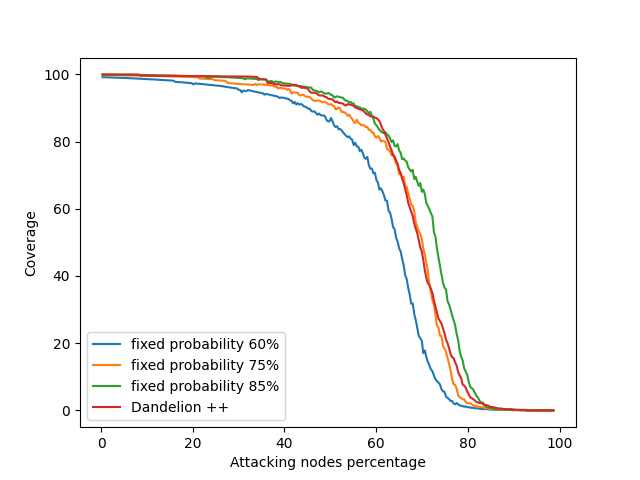
\includegraphics[width=1.1\textwidth]{pict/results/noatk-40.png}
			\centering 
			\caption{Coverage outcome under standard Sybil behaviour with a network of 40000 edges}
			\label{fig:noatk40}
        \end{minipage}
        \hspace{0.5cm}
        \begin{minipage}[b]{0.5\linewidth}
            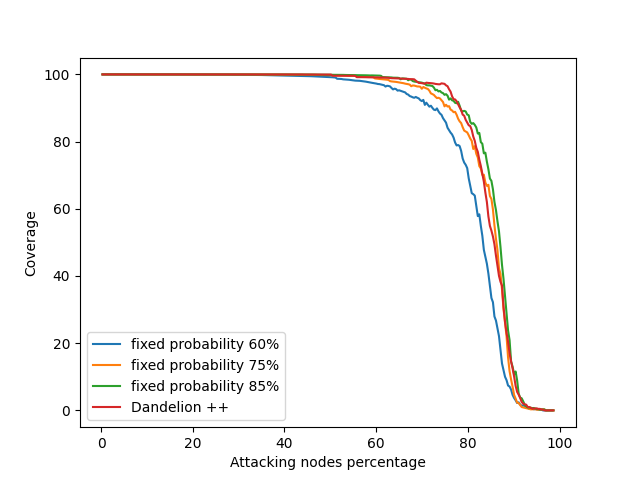
\includegraphics[width=1.1\textwidth]{pict/results/noatk-80.png}
			\centering 
			\caption{Coverage outcome under standard Sybil behaviour with a network of 80000 edges}
			\label{fig:notatk80}
        \end{minipage}
    \end{figure}

Changing the behaviour of Sybil nodes to disseminate bogus network information, as described in Section~\ref{sec:atkdetails}, yields the results shown in Fig.~\ref{fig:in-cov}. The outcome is similar for every protocol: coverage drops steeply for each of them, thus confirming the efficacy of the new behaviour. Despite achieving the best coverage in previous results, even Dandelion ++ seems ineffective.\par

\begin{figure}[h]
	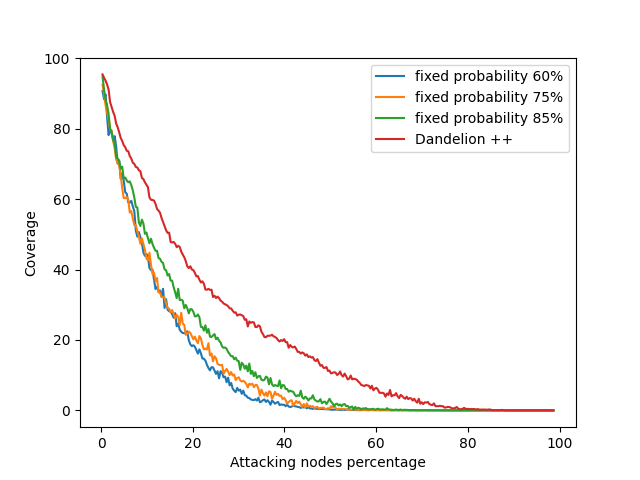
\includegraphics[width=.8\textwidth]{pict/results/in-cov.png}
	\centering 
	\caption{Coverage results}
	\label{fig:in-cov}
\end{figure}

The following metrics are reported in order to study the topology of the new network and to assess how well the new behaviour of malicious nodes has worked.

The average degree of honest nodes reveals that each node is highly connected and has on average an higher degree than those in the results of Serena et al. (Fig.~\ref{fig:degreehon}). This further confirms the efficacy of the new attack, as previous results stated the importance of dense topologies as a mean to prevent Sybil attacks.\par

    \begin{figure}[ht]
        \begin{minipage}[b]{0.5\linewidth}
            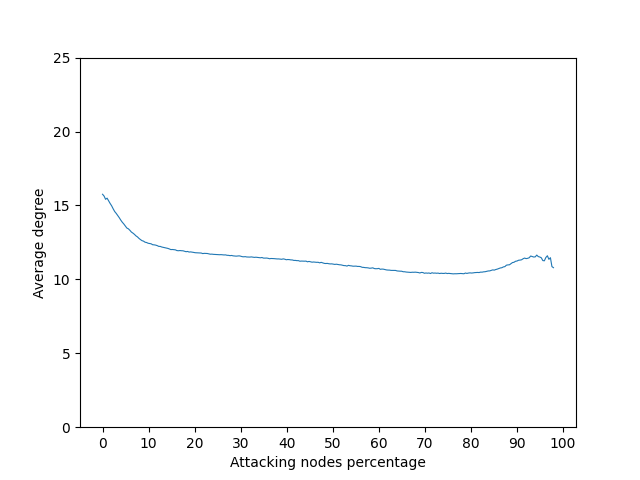
\includegraphics[width=1.1\textwidth]{pict/results/in-hon-avg-neigh.png}
			\centering
			\caption{Average degree of honest nodes (standard attack scenario)}
			\label{fig:degreehon}
        \end{minipage}
        \hspace{0.5cm}
        \begin{minipage}[b]{0.5\linewidth}
			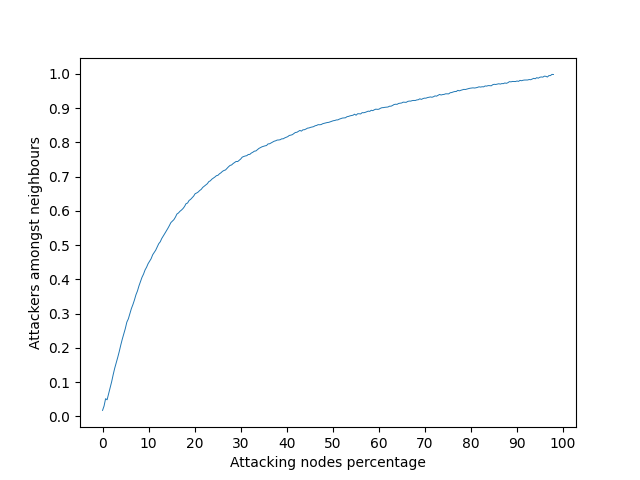
\includegraphics[width=1.1\textwidth]{pict/results/in-hon-avg-neigh-atk.png}
			\centering
			\caption{Average percentage of Sybils among neighbours (standard attack scenario)}
			\label{fig:avgatk}
        \end{minipage}
    \end{figure}


The average percentage of malicious neighbours is shown in Fig.~\ref{fig:avgatk}. It is fundamental to evaluate the efficacy of the new Sybils behaviour, as the closer they get to eclipsing honest nodes the higher the chance of carrying out a block-withholding attack would be.\par

Furthermore, the reader can see how well false network information was spread in the graph shown in Fig.~\ref{fig:avgatk-known}, as it depicts the percentage of malicious nodes in the peer cache of honest nodes. The data can also be interpreted as the probability of a node connecting to a Sybil, since new connections are chosen uniformly at random from the cache.\par

    \begin{figure}[ht]
        \begin{minipage}[b]{0.5\linewidth}
            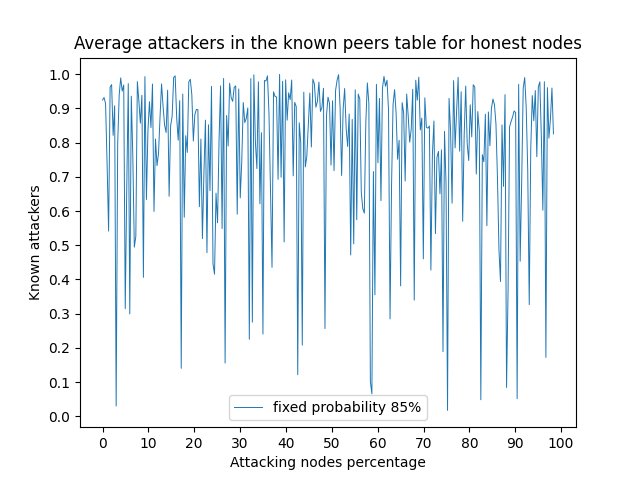
\includegraphics[width=1.1\textwidth]{pict/results/in-hon-avg-known-atk.png}
			\centering
			\caption{Average percentage of Sybils in the peer cache (standard attack scenario)}
			\label{fig:avgatk-known}
        \end{minipage}
        \hspace{0.5cm}
        \begin{minipage}[b]{0.5\linewidth}
			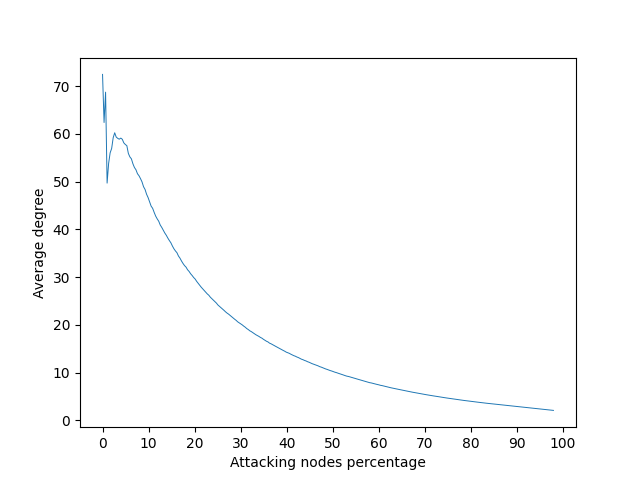
\includegraphics[width=1.1\textwidth]{pict/results/in-atk-avg-degree.png}
			\centering
			\caption{Average degree of Sybil nodes (standard attack scenario)}
			\label{fig:in-atk-degree}
        \end{minipage}
    \end{figure}
    
The average degree of malicious nodes (Fig.~\ref{fig:in-atk-degree}) shows that Sybils are far more connected than honest nodes, especially when they are fewer. This is due to the lack of an upper bound on outgoing connections.

The descending trend of the degree is due to malicious nodes avoiding making connections between themselves. When the number of attacking nodes increases, that of honest nodes decreases proportionally, thus leaving fewer nodes to connect to.

With samples of the degree distribution, Fig.~\ref{fig:incluster}, it is possible to understand how the topology of the underlying network was influenced.  Where there is a low percentage of Sybils in the network malicious nodes tend to have on average an extremely high degree. As the percentage increases the tendency to create clusters emerges: some Sybils reach extremely high degrees, whilst others are left poorly connected.\par


    \begin{figure}[ht]
        \begin{minipage}[b]{0.5\linewidth}
            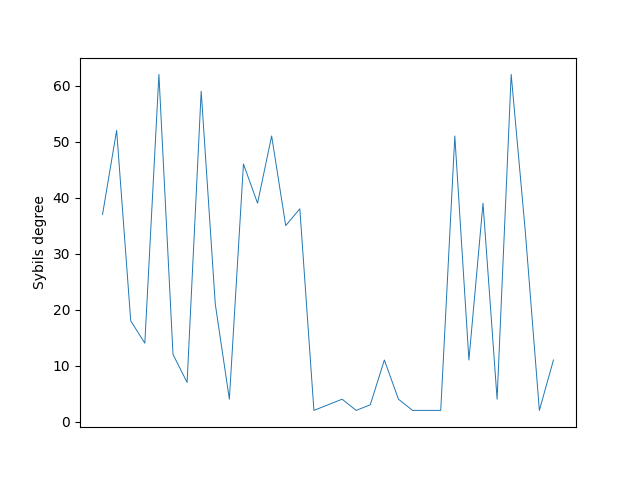
\includegraphics[width=1.1\textwidth]{pict/results/in-cluster.png}
			\centering
			\caption{Sample of degree distribution of Sybil nodes (standard attack scenario)}
			\label{fig:incluster}
        \end{minipage}
        \hspace{0.5cm}
        \begin{minipage}[b]{0.5\linewidth}
			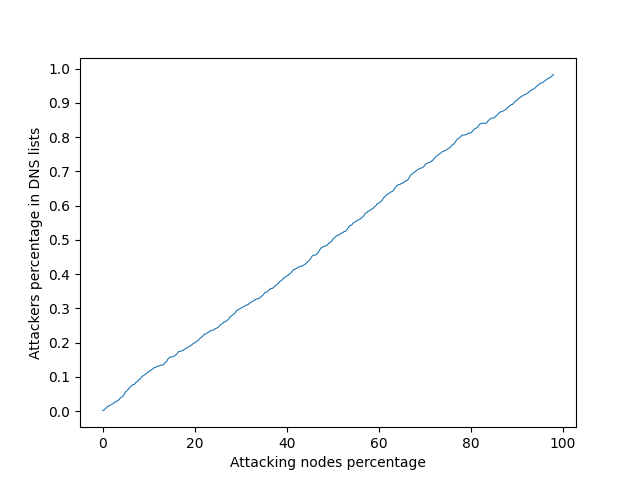
\includegraphics[width=1.1\textwidth]{pict/results/in-dns.png}
			\centering
			\caption{Percentage of Sybil nodes in the DNSs (standard attack scenario)}
			\label{fig:dns}
        \end{minipage}
    \end{figure}

Also DNSs have their role in determining the efficacy of the attack. The percentage of malicious addresses in their peer lists directly influences the chance of a node on fresh bootstrap connecting to a malicious node first. Fig.~\ref{fig:dns} shows a steady increase in the percentage of malicious addresses.

\section{Alternative attack scenario}\label{sec:external}
In the second attack scenario all malicious nodes are on fresh bootstrap and have to join the network while it is still forming. The number of attacking nodes in these simulations has been increased up to 30000. A total of 300 simulations are run, 100 attacking nodes are added at each.\par

The attack does not achieve any results in this scenario, as shown by the coverage in Fig.~\ref{fig:ext-cov}. The network is thus resistant to such Sybil attack.\par

\begin{figure}[h!]
            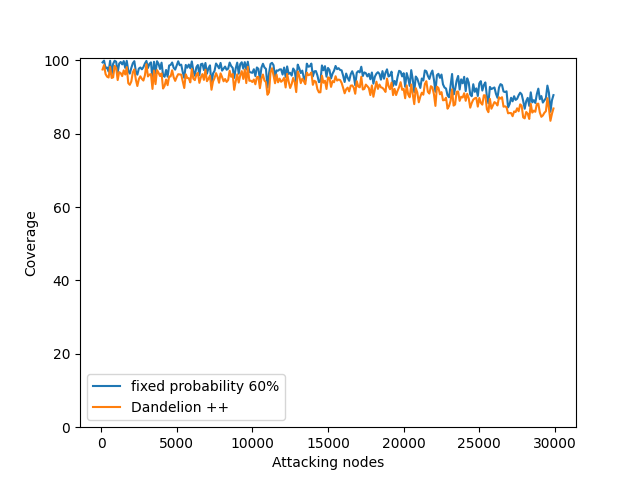
\includegraphics[width=0.8\textwidth]{pict/results/ext-cov.png}
			\centering
			\caption{Coverage with Sybils on fresh bootstrap (second attack scenario)}
			\label{fig:ext-cov}
\end{figure}

    \begin{figure}[ht]
        \begin{minipage}[b]{0.5\linewidth}
            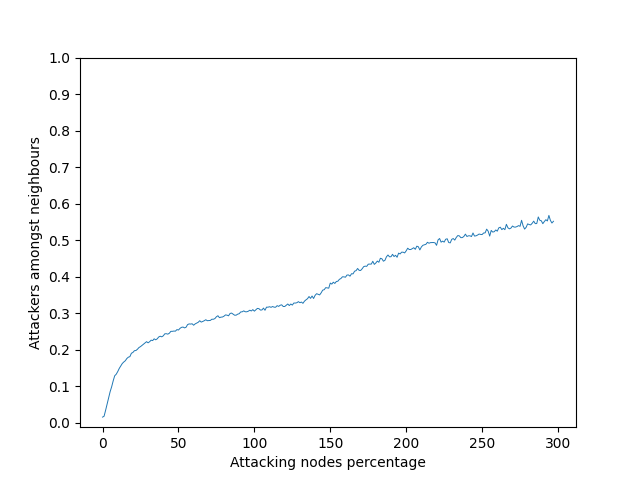
\includegraphics[width=1.1\textwidth]{pict/results/ext-hon-atk-neigh.png}
			\centering
			\caption{Percentage of Sybil neighbours in the second attack scenario}
			\label{fig:ex-atk-neigh}
        \end{minipage}
        \hspace{0.5cm}
        \begin{minipage}[b]{0.5\linewidth}
			\centering
            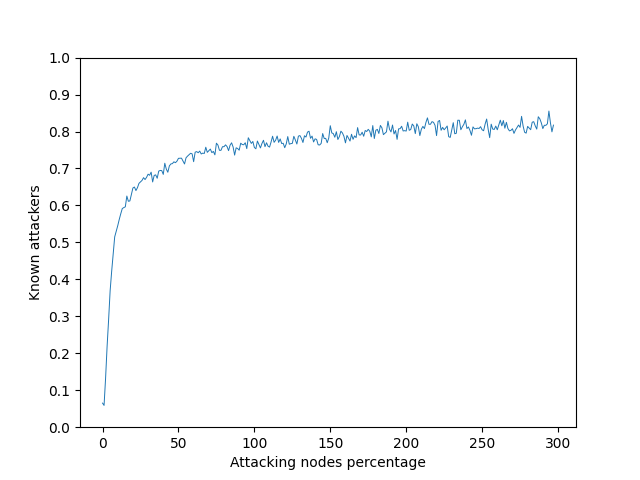
\includegraphics[width=1.1\textwidth]{pict/results/ex-hon-atk-known.png}
			\caption{Sybils average degree in the second attack scenario}
			\label{fig:ex-atk-known}
        \end{minipage}
    \end{figure}
    
    \begin{figure}[ht]
        \begin{minipage}[b]{0.5\linewidth}
            \centering
            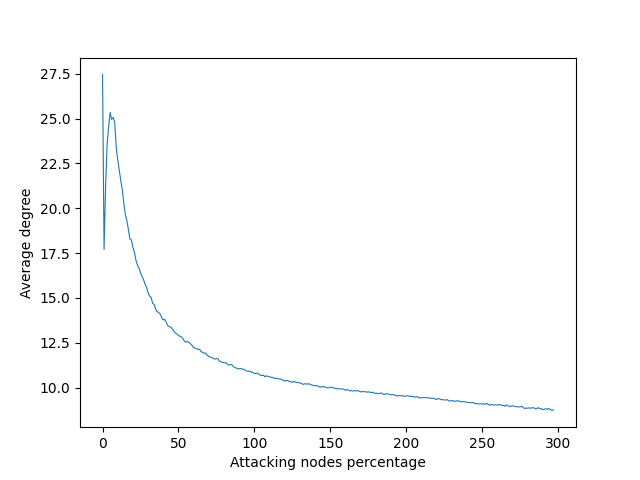
\includegraphics[width=1.1\textwidth]{pict/results/ex-atk-avg-degree.png}
			\caption{Sybils average degree in the second attack scenario}
			\label{fig:ex-atk-degree}
        \end{minipage}
        \hspace{0.5cm}
        \begin{minipage}[b]{0.5\linewidth}
			\centering
			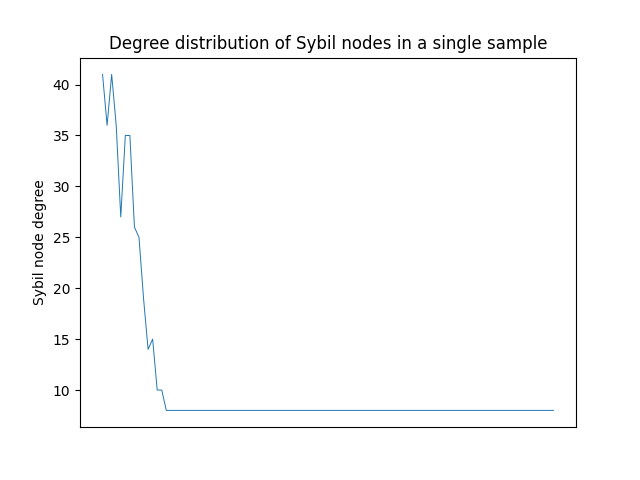
\includegraphics[width=1.1\textwidth]{pict/results/ex-atk-dd.png}
			\caption{Degree of randomly sampled nodes during the second attack scenario - nodes joining the network last have a lower degree}
			\label{fig:dd}
        \end{minipage}
    \end{figure}


Also the the changes in the behaviour of Sybils have been ineffective, since rate of malicious neighbours is significantly lower (Fig.~\ref{fig:ex-atk-neigh}).\par

Despite that, Sybils still managed to disseminate malicious addresses well, although achieving results worse than those in the previous setting (Fig.~\ref{fig:ex-atk-known}).\par

Also the shape of the graph has changed. Sybils are less connected and face the same downward trend in the average degree, Fig.~\ref{fig:ex-atk-degree}, as a result of the increasing number of attackers.

Moreover, by looking at a sample of the degree distribution, Fig.~\ref{fig:dd}, the reader can see that only the Sybils that connect first (they connect sequentially, Sec.~\ref{sec:softw}) are able to establish more connections, whereas the others are left in sparser areas of the graph.\par

In this scenario DNS peer lists did not have any attacker, since they cannot contain nodes on fresh bootstrap.